% Chapter Template

\chapter{Methodology} % Main chapter title
\label{chapter3} 

The following chapter includes methodological procedures that are common for all chapters.
More detailed methodological procedures will be described in each chapter separately. 

\section{Data}

We used UK-DALE \cite{UKDALE}, REFIT \cite{REFIT}, ECO \cite{ECO}, REDD \cite{REDD}, and iAWE \cite{iAWE}.
All datasets measured electrical energy consumption for residential buildings. 
They include main smart meter data, as well as sub-meter data for each appliance in a dwelling. 
For easier handling datasets will be sliced into 1-hour intervals. 

\begin{figure}[H]
	\centering
	\caption{Universal normalized daily usage profile for weekend and weekday for a microwave. Superposition of data from 25 homes.}
	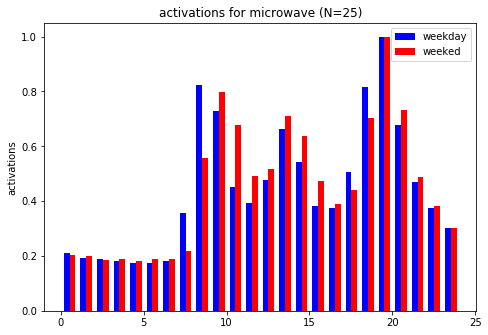
\includegraphics[width=0.9\textwidth]{../Figures/microwave_norm_n25.png}
	\label{fig:UniNormMicrowave}
\end{figure}

Data will be then used to generate various load profiles. 
One such example can be seen in Figure \ref{fig:UniNormMicrowave}. The histogram shows normalized daily 
activation for microwaves. It consists of data from 25 homes from 4 different
datasets. 

\section{Tools used}

To process the data and to obtain the results the environment and virtual machines from Google Colab (\cite{colab}) were used.
They offer access to Google GPU-accelerated compute machines with 12 GB of RAM. 
Colab also offers access to Drive cloud storage, where the dataset and results were stored.
While running the experiments, we made use of Drives 100 TB pooled cloud storage, which is available to students of the University of Ljubljana. 
For development and version control, GitHub was used. 

Within the Colab which uses a Jupyter (\cite{jupyter}) environment at its core, various python libraries were used.
To store and read the datasets in hdf5 format we used h5py  (\cite{hdf5}) and Pickle  (\cite{pickle}).
To load datasets into RAM and then handle them, the pandas  (\cite{pandas}) library was used.
For handling the large matrices and calculating we used NumPy  (\cite{numpy}).
To present the data with graphs we have used Matplotlib  (\cite{matplotlib}) and to present data with heatmap Seaborn  (\cite{seaborn}).
For easier implementation, such as of the t-SNE, a Scikit  (\cite{scikit}) and SciPy  (\cite{scipy}) libraries were used.
